\documentclass[letter, 11pt, onesided]{memoir}

\usepackage[no-math]{fontspec}
\usepackage{xpatch}
	\renewcommand{\ttdefault}{ul9}
	\xpatchcmd{\ttfamily}{\selectfont}{\fontencoding{T1}\selectfont}{}{}
	\DeclareTextCommand{\nobreakspace}{T1}{\leavevmode\nobreak\ }
\usepackage{polyglossia} % English please
	\setdefaultlanguage[variant=us]{english}
\usepackage[charter,cal=cmcal]{mathdesign} %different font
\usepackage{avant}
\usepackage{microtype} % Less badboxes

\usepackage{calc, ifthen, xparse, xspace}
\usepackage{makeidx}
\usepackage[hidelinks]{hyperref}   % Internal hyperlinks
\usepackage{mathtools} % replaces amsmath
\usepackage{etoolbox}
\usepackage{bbm} %lower case blackboard font
\usepackage{amsthm, bm}
\usepackage{graphicx}
\usepackage{xcolor}
\usepackage{multicol}
\usepackage{tikz}
	\tikzset{>=latex}
	\usetikzlibrary{calc}
	\usetikzlibrary{backgrounds}
	\usetikzlibrary{patterns,decorations.pathreplacing}
	\usetikzlibrary{spy}
\usepackage{pgfplots}
	\pgfplotsset{compat=1.12}
	\usepgfplotslibrary{colormaps}
	\usepgfplotslibrary{patchplots}
	\usepgfplotslibrary{fillbetween}
\usepackage{tcolorbox}
	\tcbuselibrary{breakable}
\usepackage[inline,shortlabels]{enumitem}
\setlistdepth{9}

\usepackage{datatool}

\usepackage{float}


\usepgfplotslibrary{external}
\tikzexternalize[prefix=tikz/]


%%% Specify the cool macros
\newcommand{\declarecommand}[1]{\providecommand{#1}{}\renewcommand{#1}}
\declarecommand{\R}{\mathbb{R}}  % we don't care if it's already defined.  We really want *this* command!
\declarecommand{\Z}{\mathbb{Z}}
\declarecommand{\Q}{\mathbb{Q}}
\declarecommand{\N}{\mathbb{N}}
\declarecommand{\C}{\mathbb{C}}
\declarecommand{\d}{\mathrm{d}}
\declarecommand{\dd}{\mathbbm{d}} % exterior derivative
\declarecommand{\P}{\mathbb{P}}
\DeclareMathOperator{\Span}{span}
\DeclareMathOperator{\Img}{img}
\DeclareMathOperator{\Id}{id}
\DeclareMathOperator{\Range}{range}
\DeclareMathOperator{\Rref}{rref}
\DeclareMathOperator{\Rank}{rank}
\DeclareMathOperator{\Speed}{speed}
\DeclareMathOperator{\Vel}{velocity}
\DeclareMathOperator{\Accel}{accel}
\DeclareMathOperator{\Null}{null}
\DeclareMathOperator{\Nullity}{nullity}
\DeclareMathOperator{\Char}{char}
\DeclareMathOperator{\Proj}{proj}
\DeclareMathOperator{\Flux}{Flux}
\DeclareMathOperator{\Circ}{Circ}
\DeclareMathOperator{\Curl}{curl}
\DeclareMathOperator{\Dim}{dim}
\DeclareMathOperator{\Perp}{perp}
\DeclareMathOperator{\Ker}{kernel}
\DeclareMathOperator{\Trans}{\downarrow\!}
\DeclareMathOperator{\Transu}{\uparrow\!}
\DeclareMathOperator{\Arclen}{arc\,len}
\newcommand{\Arclenfrom}[3]{\Arclen #1 \Big|_{#2}^{#3}}
\newcommand{\proj}{\Proj}
\newcommand{\xhat}{{\hat {\mathbf x}}}
\newcommand{\yhat}{{\hat {\mathbf y}}}
\newcommand{\zhat}{{\hat {\mathbf z}}}
\newcommand{\mat}[1]{\begin{bmatrix*}[r]#1\end{bmatrix*}}
\newcommand{\matc}[1]{\begin{bmatrix}#1\end{bmatrix}}
\newcommand{\formarg}[2]{\big(#1;\, #2\big)}
\newcommand{\abs}[1]{\left\vert #1 \right\vert}
\newcommand{\norm}[1]{\left\| #1 \right\|}
\newcommand{\inner}[2]{\langle #1, #2 \rangle}
\newcommand{\set}[1]{\left\{ #1 \right\}}
% just to make sure it exists
\providecommand\given{}
% can be useful to refer to this outside \Set
\newcommand\SetSymbol[1][]{%
	\nonscript\::%
	\allowbreak
	\nonscript\:
	\mathopen{}}
\DeclarePairedDelimiterX\Set[1]\{\}{%
	\renewcommand\given{\SetSymbol[\delimsize]}
	#1
}
\renewcommand{\it}{\itshape}
% footnote without marker
\newcommand\blfootnote[1]{%
  \begingroup
  \renewcommand\thefootnote{}\footnote{#1}%
  \addtocounter{footnote}{-1}%
  \endgroup
}


% labels for source attributions
\NewDocumentCommand{\openstax}{o}{%
	\IfNoValueTF{#1}{%
		{\color{blue}\sffamily{OS}}%
	}{%
		{\color{blue}\sffamily{OS}}%  XXX Todo, make this href to the appropriate problem number
	}\xspace%
}

% labels for source attributions
\NewDocumentCommand{\grout}{o}{%
	\IfNoValueTF{#1}{%
		{\color{blue}\sffamily{G}}%
	}{%
		{\color{blue}\sffamily{G}}%  XXX Todo, make this href to the appropriate problem number
	}\xspace%
}

% set up some deep enumerate environments for the CC license
\newlist{ccEnumerate}{enumerate}{9}
\setlist[ccEnumerate,1]{label=\alph*.}
\setlist[ccEnumerate,2]{label=\arabic*.}
\setlist[ccEnumerate,3]{label=\Alph*.}
\setlist[ccEnumerate,4]{label=\roman*.}
\setlist[ccEnumerate,5]{label=(\alph*)}
\setlist[ccEnumerate,6]{label=(\arabic*)}
\setlist[ccEnumerate,7]{label=(\Roman*)}
\setlist[ccEnumerate,8]{label=(\Alph*)}
\setlist[ccEnumerate,9]{label=(\roman*)}


% other enumerate environments
\NewDocumentCommand{\prob}{o}{%
	\IfNoValueTF{#1}{%
		\refstepcounter{enumi}%
		\item[\theenumi]%
	}{%
		\refstepcounter{enumi}%
		\item[\theenumi \textsuperscript{#1}]%
	}%
}
\newenvironment{problist}{%
	\begin{enumerate}
	}{%
	\end{enumerate}
}
% an environment to store problem solutions
\newenvironment{solution}{%
		\par\color{blue} Solution: 
	}{%
		\ignorespacesafterend
}

%\newlist{problist}{enumerate}{3}
%\setlist[problist]{label=\arabic*}


%%% Specify the colors
\definecolor{myorange}{HTML}{F29B23}
\definecolor{myred}{HTML}{D13409}
\definecolor{mypink}{HTML}{B3094F}
\definecolor{mydark}{HTML}{23112A}
\definecolor{mygreen}{HTML}{34A320}
\definecolor{myblue}{HTML}{2F8CEF}

\colorlet{chapcolor}{myred}
\colorlet{seccolor}{myorange}
\colorlet{headertext}{myred!70!white}
\colorlet{ocre}{mypink}

%%% Specify custom fonts
%\newfontfamily{\sfreg}{Fira Sans}
%\newfontfamily{\firasans}
%  [Ligatures=TeX, % recommended
%   UprightFont={* Light},
%   ItalicFont={* Light Italic},
%   BoldFont={* Medium},
%   BoldItalicFont={* Medium Italic}]
%  {Fira Sans}



%%% PAGE LAYOUT
%%%------------------------------------------------------------------------------

\setlrmarginsandblock{0.15\paperwidth}{*}{1} % Left and right margin
\setulmarginsandblock{0.15\paperwidth}{*}{1}  % Upper and lower margin
\checkandfixthelayout

%%% SECTIONAL DIVISIONS
%%%------------------------------------------------------------------------------

%\maxsecnumdepth{subsection} % Subsections (and higher) are numbered
%\setsecnumdepth{subsection}
%
%\makeatletter %
%\makechapterstyle{standard}{
%  \setlength{\beforechapskip}{0\baselineskip}
%  \setlength{\midchapskip}{1\baselineskip}
%  \setlength{\afterchapskip}{8\baselineskip}
%  \renewcommand{\chapterheadstart}{\vspace*{\beforechapskip}}
%  \renewcommand{\chapnamefont}{\centering\normalfont\Large}
%  \renewcommand{\printchaptername}{\chapnamefont \@chapapp}
%  \renewcommand{\chapternamenum}{\space}
%  \renewcommand{\chapnumfont}{\normalfont\Large}
%  \renewcommand{\printchapternum}{\chapnumfont \thechapter}
%  \renewcommand{\afterchapternum}{\par\nobreak\vskip \midchapskip}
%  \renewcommand{\printchapternonum}{\vspace*{\midchapskip}\vspace*{5mm}}
%  \renewcommand{\chaptitlefont}{\centering\bfseries\LARGE}
%  \renewcommand{\printchaptertitle}[1]{\chaptitlefont ##1}
%  \renewcommand{\afterchaptertitle}{\par\nobreak\vskip \afterchapskip}
%}
%\makeatother
%
%\chapterstyle{standard}

%\setsecheadstyle{\normalfont\large\bfseries}
%\setsubsecheadstyle{\normalfont\normalsize\bfseries}
%\setparaheadstyle{\normalfont\normalsize\bfseries}
%\setparaindent{0pt}\setafterparaskip{0pt}

\renewcommand{\chapnumfont}{\normalfont\huge\sffamily\bfseries}
\renewcommand{\chaptitlefont}{\color{chapcolor}\chapnumfont\mdseries}
\renewcommand{\printchaptername}{\chapnumfont Chapter}
\makeatletter
	\renewcommand{\hangsecnum}{%
	  \def\@seccntformat##1{%
	    \makebox[0pt][r]{%
	      \color{seccolor}%
	      \csname the##1\endcsname
	      \quad
	    }%
	  }%
	}
\makeatother
%\setsecnumformat{\llap{\color{seccolor}\csname the#1\endcsname\quad}}

\setsecheadstyle{\Large\bfseries\sffamily\raggedright}
\setsubsecheadstyle{\large\sffamily\raggedright}
\setsubsubsecheadstyle{\normalsize\sffamily\raggedright}
\setsechook{\hangsecnum}
\setsubsechook{\defaultsecnum}
\setsubsubsechook{\defaultsecnum}


\makeatletter
	\setlength{\headwidth}{\textwidth}
	%\addtolength{\headwidth}{\marginparsep}
	%\addtolength{\headwidth}{\marginparwidth}
	\makepagestyle{serifpage}
	\makerunningwidth{serifpage}{\headwidth}
	\makeheadrule{serifpage}{\headwidth}{\normalrulethickness}
	\makeheadposition{serifpage}{flushright}{flushleft}{}{}
	\makepsmarks{serifpage}{%
		\let\@mkboth\markboth
		\def\chaptermark##1{\markboth{\textsf{\color{headertext}##1}}{\textsf{\color{headertext}##1}}}% % left & right marks
		\def\sectionmark##1{\markright{%
		\ifnum \c@secnumdepth>\z@
			{\color{seccolor}\sffamily\thesection\ }
		\fi
		\textsf{\color{headertext}##1}}}
	}
	\makeevenhead{serifpage}%
		{\normalfont\sffamily\thepage}{}{\normalfont\sffamily \leftmark}
	\makeoddhead{serifpage}%
		{\normalfont\sffamily \rightmark}{}{\normalfont\sffamily\thepage}
\makeatother

\pagestyle{serifpage}

%%% Theorem Environments

\makeatletter
	\newcommand{\intoo}[2]{\mathopen{]}#1\,;#2\mathclose{[}}
	\newcommand{\ud}{\mathop{\mathrm{{}d}}\mathopen{}}
	\newcommand{\intff}[2]{\mathopen{[}#1\,;#2\mathclose{]}}
	\newtheorem{notation}{Notation}[chapter]

	%%%%%%%%%%%%%%%%%%%%%%%%%%%%%%%%%%%%%%%%%%%%%%%%%%%%%%%%%%%%%%%%%%%%%%%%%%%
	%%%%%%%%%%%%%%%%%%%% dedicated to boxed/framed environements %%%%%%%%%%%%%%
	%%%%%%%%%%%%%%%%%%%%%%%%%%%%%%%%%%%%%%%%%%%%%%%%%%%%%%%%%%%%%%%%%%%%%%%%%%%
	\newtheoremstyle{orangenumbox}% % Theorem style name
	{0pt}% Space above
	{0pt}% Space below
	{\normalfont}% % Body font
	{}% Indent amount
	{\small\bfseries\sffamily\color{myorange}}% % Theorem head font
	{\;}% Punctuation after theorem head
	{0.25em}% Space after theorem head
	{\small\sffamily\color{myorange!80!black}\thmname{#1}\nobreakspace\thmnumber{\@ifnotempty{#1}{}\@upn{#2}}% Theorem text (e.g. Theorem 2.1)
	\thmnote{\nobreakspace\the\thm@notefont\sffamily\bfseries\color{black}---\nobreakspace#3.}} % Optional theorem note
	\renewcommand{\qedsymbol}{$\blacksquare$}% Optional qed square

	\newtheoremstyle{ocrenumbox}% % Theorem style name
	{0pt}% Space above
	{0pt}% Space below
	{\normalfont}% % Body font
	{}% Indent amount
	{\small\bfseries\sffamily\color{ocre}}% % Theorem head font
	{\;}% Punctuation after theorem head
	{0.25em}% Space after theorem head
	{\small\sffamily\color{ocre}\thmname{#1}\nobreakspace\thmnumber{\@ifnotempty{#1}{}\@upn{#2}}% Theorem text (e.g. Theorem 2.1)
	\thmnote{\nobreakspace\the\thm@notefont\sffamily\bfseries\color{black}---\nobreakspace#3.}} % Optional theorem note
	\renewcommand{\qedsymbol}{$\blacksquare$}% Optional qed square

	\newtheoremstyle{blacknumex}% Theorem style name
	{5pt}% Space above
	{5pt}% Space below
	{\normalfont}% Body font
	{} % Indent amount
	{\small\bfseries\sffamily}% Theorem head font
	{\;}% Punctuation after theorem head
	{0.25em}% Space after theorem head
	{\small\sffamily{\tiny\ensuremath{\blacksquare}}\nobreakspace\thmname{#1}\nobreakspace\thmnumber{\@ifnotempty{#1}{}\@upn{#2}}% Theorem text (e.g. Theorem 2.1)
	\thmnote{\nobreakspace\the\thm@notefont\sffamily\bfseries---\nobreakspace#3.}}% Optional theorem note

	\newtheoremstyle{blacknumbox} % Theorem style name
	{0pt}% Space above
	{0pt}% Space below
	{\normalfont}% Body font
	{}% Indent amount
	{\small\bfseries\sffamily}% Theorem head font
	{\;}% Punctuation after theorem head
	{0.25em}% Space after theorem head
	{\small\sffamily\thmname{#1}\nobreakspace\thmnumber{\@ifnotempty{#1}{}\@upn{#2}}% Theorem text (e.g. Theorem 2.1)
	\thmnote{\nobreakspace\the\thm@notefont\sffamily\bfseries---\nobreakspace#3.}}% Optional theorem note

	%%%%%%%%%%%%%%%%%%%%%%%%%%%%%%%%%%%%%%%%%%%%%%%%%%%%%%%%%%%%%%%%%%%%%%%%%%%
	%%%%%%%%%%%%% dedicated to non-boxed/non-framed environments %%%%%%%%%%%%%%
	%%%%%%%%%%%%%%%%%%%%%%%%%%%%%%%%%%%%%%%%%%%%%%%%%%%%%%%%%%%%%%%%%%%%%%%%%%%
	\newtheoremstyle{ocrenum}% % Theorem style name
	{5pt}% Space above
	{5pt}% Space below
	{\normalfont}% % Body font
	{}% Indent amount
	{\small\bfseries\sffamily\color{ocre}}% % Theorem head font
	{\;}% Punctuation after theorem head
	{0.25em}% Space after theorem head
	{\small\sffamily\color{ocre}\thmname{#1}\nobreakspace\thmnumber{\@ifnotempty{#1}{}\@upn{#2}}% Theorem text (e.g. Theorem 2.1)
	\thmnote{\nobreakspace\the\thm@notefont\sffamily\bfseries\color{black}---\nobreakspace#3.}} % Optional theorem note
	\renewcommand{\qedsymbol}{$\blacksquare$}% Optional qed square

    \newtheoremstyle{bluenum}% % Theorem style name
	{5pt}% Space above
	{5pt}% Space below
	{\normalfont}% % Body font
	{}% Indent amount
	{\small\bfseries\sffamily\color{myblue}}% % Theorem head font
	{\;}% Punctuation after theorem head
	{0.25em}% Space after theorem head
	{\small\sffamily\color{myblue}\thmname{#1}\nobreakspace\thmnumber{\@ifnotempty{#1}{}\@upn{#2}}% Theorem text (e.g. Theorem 2.1)
	\thmnote{\nobreakspace\the\thm@notefont\sffamily\bfseries\color{black}---\nobreakspace#3.}} % Optional theorem note
	\renewcommand{\qedsymbol}{$\blacksquare$}% Optional qed square

    \newtheoremstyle{greennum}% % Theorem style name
	{5pt}% Space above
	{5pt}% Space below
	{\normalfont}% % Body font
	{}% Indent amount
	{\small\bfseries\sffamily\color{mygreen}}% % Theorem head font
	{\;}% Punctuation after theorem head
	{0.25em}% Space after theorem head
	{\small\sffamily\color{mygreen}\thmname{#1}\nobreakspace\thmnumber{\@ifnotempty{#1}{}\@upn{#2}}% Theorem text (e.g. Theorem 2.1)
	\thmnote{\nobreakspace\the\thm@notefont\sffamily\bfseries\color{black}---\nobreakspace#3.}} % Optional theorem note
	\renewcommand{\qedsymbol}{$\blacksquare$}% Optional qed square
	\makeatother

	% Defines the theorem text style for each type of theorem to one of the three styles above
	\newcounter{dummy}
	\numberwithin{dummy}{section}
	\theoremstyle{orangenumbox}
	\newtheorem{theoremeT}[dummy]{Theorem}
	\theoremstyle{ocrenumbox}
	\newtheorem{problem}{Problem}[chapter]
	\newtheorem{exerciseT}{Exercise}[chapter]
	\theoremstyle{blacknumex}
	\newtheorem{exampleT}{Example}[chapter]
	\theoremstyle{blacknumbox}
	\newtheorem{vocabulary}{Vocabulary}[chapter]
	\newtheorem{definitionT}{Definition}[section]
	\newtheorem{corollaryT}[dummy]{Corollary}
	\theoremstyle{bluenum}
	\newtheorem{propositionT}[dummy]{Proposition}
    \theoremstyle{greennum}
    \newtheorem*{proofT}{Proof}

	%----------------------------------------------------------------------------------------
	%	DEFINITION OF COLORED BOXES
	%----------------------------------------------------------------------------------------

	\RequirePackage[framemethod=default]{mdframed} % Required for creating the theorem, definition, exercise and corollary boxes

	% Theorem box
	\newmdenv[skipabove=7pt,
	skipbelow=7pt,
	rightline=false,
	leftline=true,
	topline=false,
	bottomline=false,
	backgroundcolor=myorange!20,
	linecolor=myorange,
	innerleftmargin=5pt,
	innerrightmargin=5pt,
	innertopmargin=5pt,
	innerbottommargin=5pt,
	leftmargin=0cm,
	rightmargin=0cm,
	linewidth=4pt]{tBox}

	% Exercise box
	\newmdenv[skipabove=7pt,
	skipbelow=7pt,
	rightline=false,
	leftline=true,
	topline=false,
	bottomline=false,
	backgroundcolor=ocre!10,
	linecolor=ocre,
	innerleftmargin=5pt,
	innerrightmargin=5pt,
	innertopmargin=5pt,
	innerbottommargin=5pt,
	leftmargin=0cm,
	rightmargin=0cm,
	linewidth=4pt]{eBox}

	% Definition box
	\newmdenv[skipabove=7pt,
	skipbelow=7pt,
	rightline=false,
	leftline=true,
	topline=false,
	bottomline=false,
	linecolor=ocre,
	innerleftmargin=5pt,
	innerrightmargin=5pt,
	innertopmargin=0pt,
	leftmargin=0cm,
	rightmargin=0cm,
	linewidth=4pt,
	innerbottommargin=0pt]{dBox}

	% Corollary box
	\newmdenv[skipabove=7pt,
	skipbelow=7pt,
	rightline=false,
	leftline=true,
	topline=false,
	bottomline=false,
	linecolor=gray,
	backgroundcolor=black!5,
	innerleftmargin=5pt,
	innerrightmargin=5pt,
	innertopmargin=5pt,
	leftmargin=0cm,
	rightmargin=0cm,
	linewidth=4pt,
	innerbottommargin=5pt]{cBox}

	% Exercises box
	\newmdenv[skipabove=7pt,
	skipbelow=7pt,
	rightline=false,
	leftline=false,
	topline=false,
	bottomline=false,
	linecolor=gray,
	backgroundcolor=blue!5,
	innerleftmargin=5pt,
	innerrightmargin=18pt,
	innertopmargin=0pt,
	innerbottommargin=6pt,
	leftmargin=0cm,
	rightmargin=0cm,
	linewidth=4pt]{exsBox}

    % Propositions box
    \newmdenv[skipabove=7pt,
	skipbelow=7pt,
	rightline=false,
	leftline=true,
	topline=false,
	bottomline=false,
	backgroundcolor=myblue!20,
	linecolor=myblue,
	innerleftmargin=5pt,
	innerrightmargin=5pt,
	innertopmargin=0pt,
	innerbottommargin=5pt,
	leftmargin=0cm,
	rightmargin=0cm,
	linewidth=4pt]{pBox}

    % Proof box (not a real box)
    \newmdenv[skipabove=7pt,
	skipbelow=7pt,
	rightline=false,
	leftline=true,
	topline=false,
	bottomline=false,
	backgroundcolor=white,
	linecolor=mygreen,
	innerleftmargin=5pt,
	innerrightmargin=5pt,
	innertopmargin=0pt,
	innerbottommargin=5pt,
	leftmargin=0cm,
	rightmargin=0cm,
	linewidth=4pt]{pfBox}

\makeatother

% Creates an environment for each type of theorem and assigns it a theorem text style from the "Theorem Styles" section above and a colored box from above
\newenvironment{theorem}{\begin{tBox}\begin{theoremeT}}{\end{theoremeT}\end{tBox}}
\renewenvironment{proof}{\begin{pfBox}\begin{proofT}}{\end{proofT}\end{pfBox}}
\newenvironment{exercise}{\begin{eBox}\begin{exerciseT}}{\end{exerciseT}\end{eBox}}
%\newenvironment{exercise}{\begin{eBox}\begin{exerciseT}}{\hfill{\color{ocre}\tiny\ensuremath{\blacksquare}}\end{exerciseT}\end{eBox}}
\newenvironment{definition}{\begin{dBox}\begin{definitionT}}{\end{definitionT}\end{dBox}}
\newenvironment{example}{\begin{exampleT}}{\hfill{\tiny\ensuremath{\blacksquare}}\end{exampleT}}
\newenvironment{corollary}{\begin{cBox}\begin{corollaryT}}{\end{corollaryT}\end{cBox}}
\newenvironment{proposition}{\begin{pBox}\begin{propositionT}}{\end{propositionT}\end{pBox}}

\newenvironment{exercises}{%
	\begin{multicols*}{2}[\begin{exsBox}{\subsection*{Exercises for \thesection}}\vspace{-0pt}\end{exsBox}]\small %
	}{%
	\end{multicols*}%
	\clearpage
}
\newenvironment{answer}{\begin{quote}}{\end{quote}}


%%% THE DOCUMENT
%%% Where all the important stuff is included!
%%%-----------------------------------------------------------------------------------------------------
\author{Bailey Bjornstad}
\title{Mathematical Fragility: An Investigation on Birth and Death Chains}

\renewcommand{\maketitlehooka}{\color{chapcolor}\chapnumfont\Huge}
\renewcommand{\maketitlehookb}{\color{black}\normalfont}
\renewcommand{\maketitlehookc}{\small
	\begin{center}
		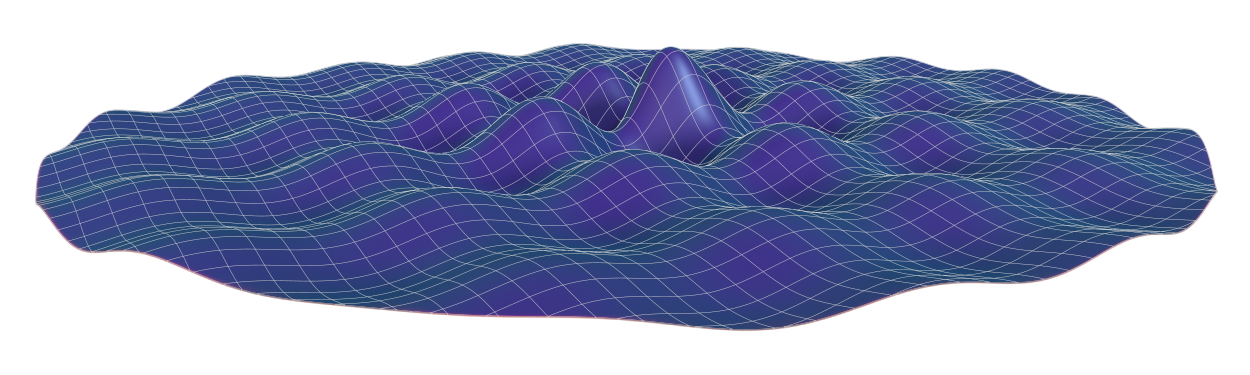
\includegraphics[width=6in]{resources/cover-render-lines-lowres.png}
	\end{center}
}
\renewcommand{\maketitlehookd}{
	\begin{center}
		
\includegraphics[width=1in]{resources/doclicense-CC-by-sa.pdf}
	\end{center}
}

\begin{document}

\frontmatter
\begin{titlingpage}
    \calccentering{\unitlength}
    \begin{adjustwidth*}{\unitlength}{-\unitlength}
        \maketitle
    \end{adjustwidth*}
\end{titlingpage}

\tableofcontents*

\mainmatter
\chapter{Introduction and Mathematical Context}
    In order to consider any conception of mathematical fragility, we must first begin to develop the
mathematical context of this project. The following discussion takes place in a probability space, and I
will leave I chose to investigate a special subset of Markov chains known as
birth and death chains. In particular, a Markov chain is defined as follows.
\begin{definition}
    A random process $X(t)$ is called a \emph{Markov chain} if, for any $t_1 < t_2$,
    \[
        P[X(t_2) \leq x \mid X(t) \text{ with } -\infty < t \in \leq t_1] = P[X(t_2) \leq x \mid X(t_1)]   
    \]
\end{definition}
In less formal terms, the probability that the chain assumes a state less than $x$ depends only on the
previous state, and none of the states before it. A birth and death chain is a special subset of Markov
chains in which the probability of stepping away from state $i$ is dependent on the current position of
the chain. A birth and death chain can be thought of as a model of a person walking amidst a fog that
obscures a point of interest. The current state of the chain is thus the current position of the walker.
For the purposes of this project, it made the most sense to consider chains with a state space of $\N$,
as they offered the most simplicity for initial investigation. The following diagram represents a birth
and death chain with state space $\N$.

\noindent
\begin{figure}[H]
    \begin{center}
        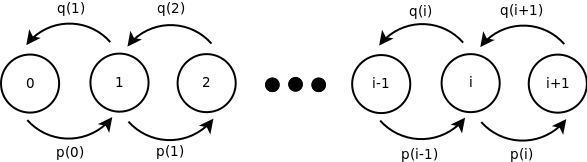
\includegraphics[width=\textwidth]{plots/birthdeathdia.png}
    \end{center}
\end{figure}

Birth and death chains are suitable context for this project due to the fact that they can model a wide
range of scenarios in a variety of different fields. Thus, mathematical fragility developed for
arbitrary birth and death chains will allow the conception of fragility to be applied in real world
scenarios. Further, there are a number of quantities associated with birth and death chains that could
provide information about the perceived fragility of these chains.

\chapter{Recurrence of Birth and Death Chains}
    It is reasonable to consider the ``fragility'' of a birth and death chain through the lens of
recurrence, a mathematical property of Markov chains that categorizes states of a chain based on whether
the chain is expected to return to that state. Further, in the case of chains with infinite states---a
birth and death chain where the states are values of $\N$, for instance---a distinction is drawn between
those states where the expected return time is infinite, and those where the expected return time is
finite.  States are thus called \emph{null-recurrent} or \emph{positive-recurrent}, respectively. In
contrast, a state is called \emph{transient} if the chain cannot be expected to return.

This allows a mathematical characterization of instances in which the chain seems to ``get lost'' from
the origin. For instance, if the origin is classified as a transient state, then a walker starting at
the origin cannot be expected to return to the origin (he may, but not with full probability). In
contrast, if the origin were classified as a recurrent state, then the walker will return with
probability $1$.  Further, if the origin were null-recurrent, the walker may find himself diverging from
the origin for arbitrary periods of time, but will with probability $1$ eventually return. If the origin
were positive-recurrent, then a concrete estimate can be placed on the walker's return time to the
origin.  This is to say that transient states are the ``most lost,'' as there can be no concrete
expectations about a walker's return to such states, nor can concrete estimates be made about how long
returning may take.  Null-recurrent states are still ``somewhat lost,'' though less so than transient
states due to the fact that concrete expectations \emph{can} be made about a walker's return.
Positive-recurrent states are the "least lost'' since a walker can be expected to return within a finite
amount of time.

In order to investigate how recurrence properties impact a chain's ``fragility,'' I first needed to
analyze some specific examples of birth and death chains. In particular, I defined a chain in which the
state-space---the possible positions that the chain can take---is the integers. Then, let
\[
    p(x) = \begin{cases}
        \frac{1}{2+\abs{x}^{-\beta}} & \text{if } x > 0 \\
        1 - \frac{1}{2+\abs{x}^{-\beta}} & \text{if } x < 0 \\
        \frac{1}{2} & \text{if } x = 0
    \end{cases}.
\]
for some $\beta >= 0$, and let $q(x) = 1 - p(x)$. Let $r(x) = 0$. This represents a birth and death
chain that is somewhat biased towards the origin, and in which the limiting probabilities
\[
    \lim_{x \to \infty} p(x) = \lim_{x \to \infty} q(x) = \frac{1}{2}  
\]
and
\[
    \lim_{x \to -\infty} p(x) = \lim_{x \to -\infty} q(x) = \frac{1}{2}.  
\]
Physically, this should represent that a walker at extremely far distances from the origin cannot see
it, and so should step either in the positive direction or in the negative direction with probability
$1/2$. We will refer to this birth and death chain as the \emph{power-distributed birth and death chain}
with parameter $\beta$.

Unfortunately, unlike in the case of stationary Markov chains in which probabilities are independent of
the position---which usually simplifes analysis---the recurrence properties of this birth and death
chain will need to be investigated a different way. I hypothesize, in particular, that if $\beta < 1$,
then the origin in the above chain will be a positive-recurrent state, and that if $\beta > 1$, then the
origin will be a null-recurrent state. In order to develop a stronger intuition about this behavior, I
turned to some numerical simulations in Python, using the NumPy and Matplotlib libraries.

I began by writing a base-class that represents a random walk, from which more specific instances can be
derived. I then developed a birth and death class inherited from the random walk base class. This
implemented the specific probability distribution detailed above. Then, for each $\beta$ in a range of
$\beta$ values---defined by a minimum $\beta$, maximum $\beta$, and $\beta$ step-size---a simulation of
one-million time steps was run, with the origin as the initial position, and the given probability
distributions. Then, using the fact that storage of return times is implemented in the random walk
class, the mean and standard-deviation of the return times was calculated, and plotted using
Matplotlib's \texttt{pyplot} class. In particular, I used the scatter-plot, histogram, and 2-dimensional
histogram functions.

For example, the following plot shows the mean return times of a simulation with $\beta$ values ranging
from $0$ to $3$ with a increments of $0.005$.

\noindent
\begin{figure}[H]
    \begin{center}
        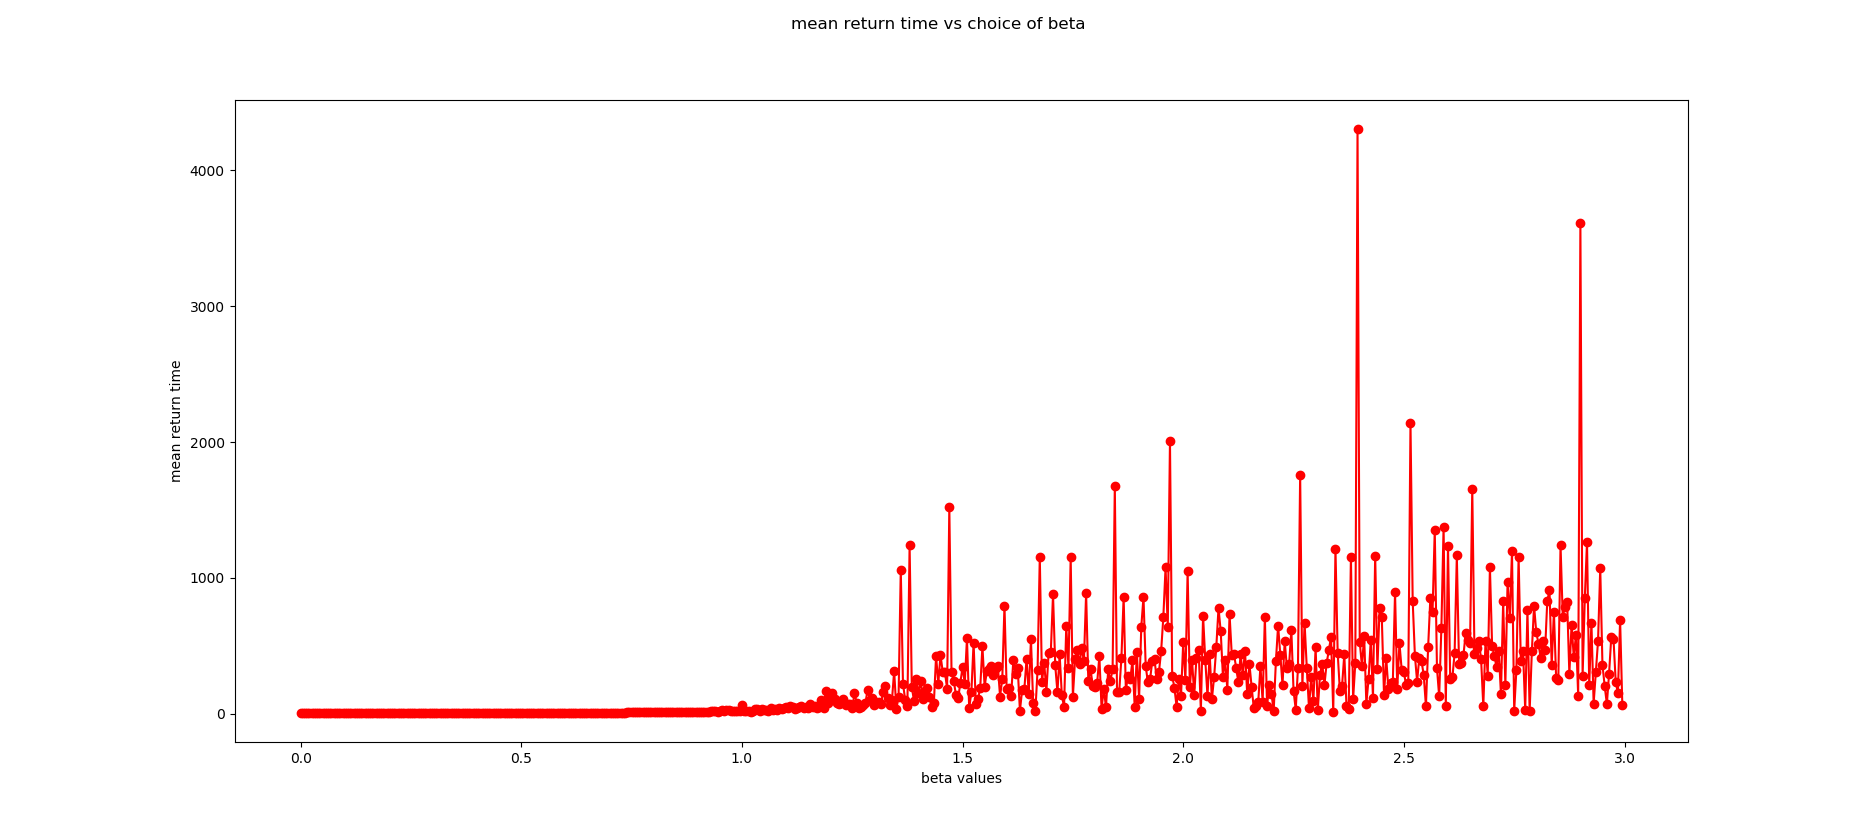
\includegraphics[width=\textwidth]{plots/returntimesplot1.png}
    \end{center}
\end{figure}

Here, it appears as though the mean return times begin to scatter into higher values shortly after
$\beta$ grows beyond $1$, thus supporting that the chains may be getting ``more lost'' more frequently.
This suggests that the origin in the given birth and death chain may be either null-recurrent or
transient when $\beta > 1$ and is, in contrast, positive-recurrent when $\beta < 1$. The corresponding
$2$-dimensional histogram similarly supports this conclusion.

\noindent
\begin{figure}[H]
    \begin{center}
        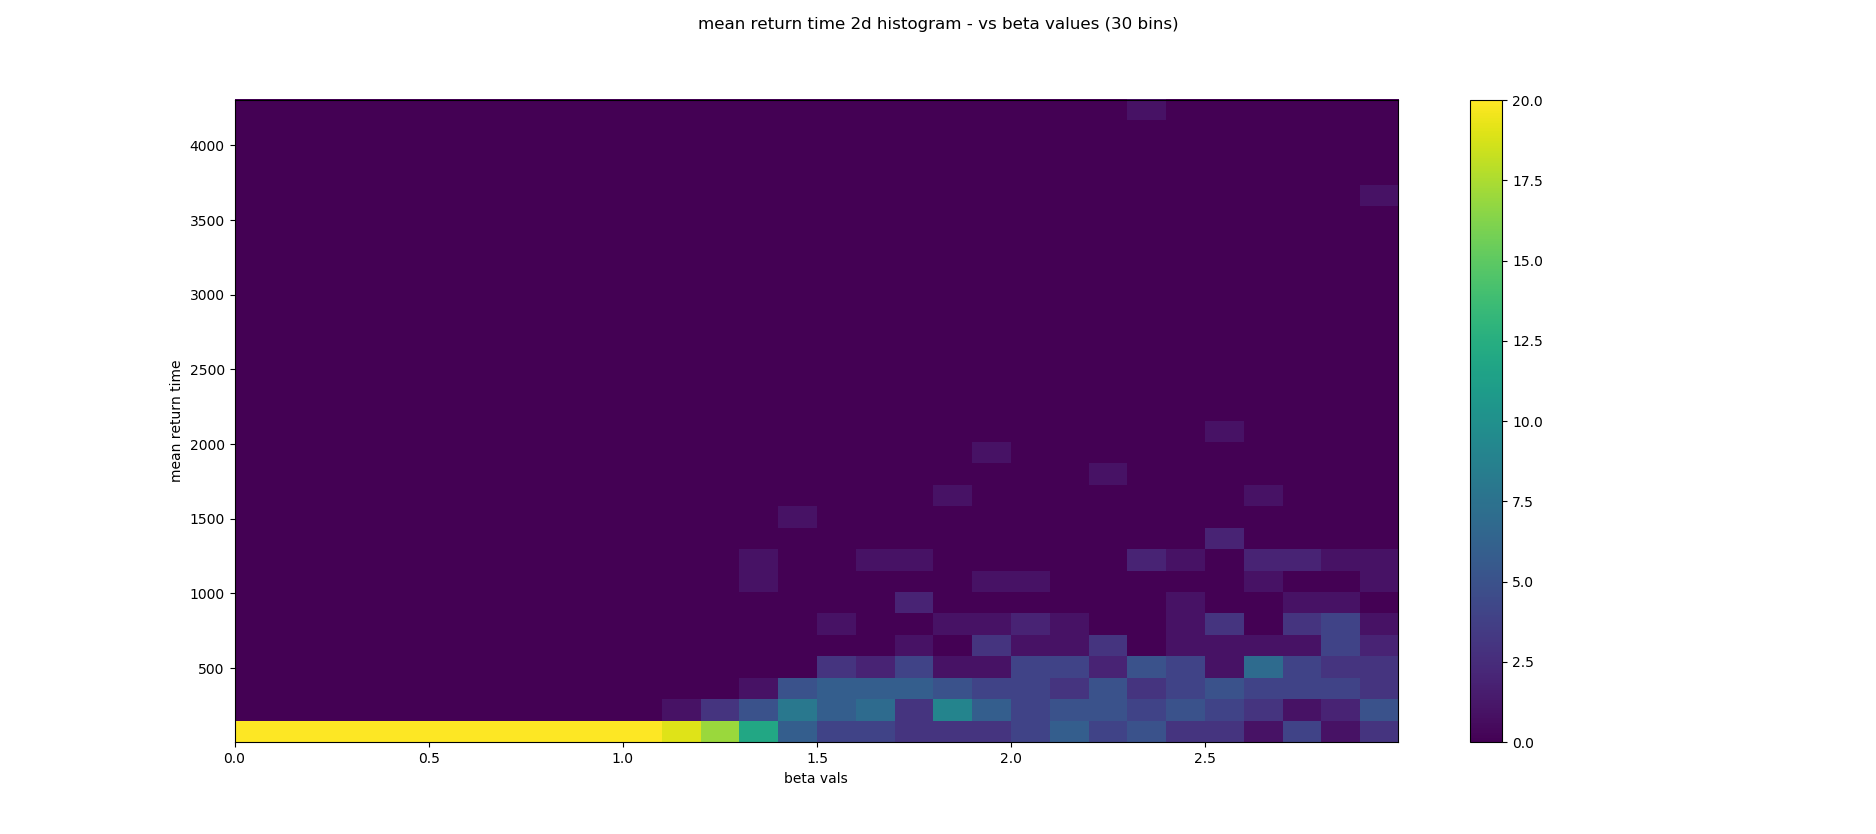
\includegraphics[width=\textwidth]{plots/returntimesplot2.png}
    \end{center}
\end{figure}

However, this is not evidence enough to support the claim, especially in mathematics where the standard
of proof lies beyond statistical inference. As such, I turned my attention toward proving the
conjucture, using a variety of analytical tools. According to Kobayashi's \emph{Probability, Random
Processes, and Statistical Analysis}, we mathematically define a recurrent or transient state the
following way. Begin by defining the \emph{first-passage time} $T_{ij}$ as the number of time steps it
takes for the chain to transition from state $i$ to state $j$. Then, we let $\rho_{ij}^{(n)}$ be the
probability that $T_{ij} = n$; in other words, $\rho_{ij}^{(n)} = P(T_{ij} = n)$. Thus, the follwing sum
\[
    \rho_{ij} = \sum_{n=1}^{\infty} \rho_{ij}^{(n)}  
\]
represents the probability that the chain ever starts at state $i$ and transitions to state $j$. Of
particular importance is the quantity $\rho_{ii}$, the probability that the chain ever returns to state
$i$ after first beginning there. From this, we can classify states.
\begin{definition}
    A state $i$ in the state space $\mathcal{S}$ is \emph{transient} if $\rho_{ii} < 1$ and is
    \emph{recurrent} if $\rho_{ii} = 1$.
\end{definition}
However, computation of $f_{ii}$ for any fixed state $i$ proved difficult with the distribution given
above.  Unfortunately, the position-dependence of $p(x)$ and $q(x)$ make combinatoric approaches highly
challenging, and I had to turn my attention elsewhere.

Observe, first, that $p(x) = q(-x)$ when $x > 0$. As a result, the birth and death chain is symmetric
about the origin. Further, since states change in integer increments, if the chain begins to observe
positive values, it must do so at least until the chain returns to the origin. Due to these two facts,
the given birth and death chain can be considered as if it had state space $\N$ instead of $\Z$. Thus,
it suffices to consider the birth and death chain on $\N$ with probability distribution given by
\[
    p(x) = \begin{cases}
        1 & \text{if } x = 0 \\
        \frac{1}{2+x^{-\beta}} & \text{if } x > 0
    \end{cases},
\]
and $q(x) = 1 - p(x)$. In particular, $p(0) = 1$ since $r(0) = 0$ and $q(0) = 0$ by definition.

Importantly, a new concept must be introducted: that of \emph{communication} between states. The
definition comes from Kobayashi.
\begin{definition}
    Let $i$ and $j$ be states. State $j$ is \emph{reachable} from state $i$ if there exists some $m \in
    \N$ so that the quantity $P_{ij}^{(m)} = \P[X_{n+m} = j \mid X_n =i] > 0$, and is denoted $i \to j$.
    If $i \to j$ and $j \to i$, then the states $i$ and $j$ \emph{communicate}, denoted $i
    \leftrightarrow j$.
\end{definition}
It is a common fact of Markov chains that the relation defined by communication is an equivalence
relation on the state space. Further, it is another common fact that all states in a particular
equivalence class defined by communication must be of the same type. This is to say that if $i$ and $j$
belong to the same equivalence class $\mathcal{C}$, and $i$ is a recurrent state, then $j$ is also a
recurrent state (or vice-versa). Further, we define the concept of \emph{irreducibility}.
\begin{definition}
    Let $\mathcal{C}$ be a set of states. $\mathcal{C}$ is \emph{irreducible} if $i \leftrightarrow j$
    for every $i$ and $j$ in $\mathcal{C}$.
\end{definition}

I claim that the birth and death chain with the given probability distribution is an irreducible chain.
\begin{proposition}
    The birth and death chain with probability distribution given by
    \[
        p(x) = \begin{cases}
            1 & \text{if } x = 0 \\
            \frac{1}{2+x^{-\beta}} & \text{if } x > 0
        \end{cases},
    \]
    $q(x) = 1-x$ and $r(x) = 0$ is irreducible.
\end{proposition}
\begin{proof}
    Note that for every state $i$ with $i > 0$, the quantities $p(i)$ and $q(i)$ are both positive.
    Now, fix arbitrary states $i$ and $j$, and without loss of generality suppose that $j > i$ and that
    $i \neq 0$ and $j \neq 0$. We wish to show that there exists some $m$ so that $P_{ij}^{(m)} =
    \P[X_{n+m} = j \mid X_n = i]$. Let $m = j-i$. Then, 
    \[
        P_{ij}^{(m)} = p(i)\, p(i+1)\, p(i+2)\, \cdots \, p(i+(j-i)).
    \]
    However, since all terms in this product are positive, so must be the product, so that $P_{ij}^{(m)}
    > 0$, so that $i \to j$. Similarly,
    \[
        P_{ji}^{(m)} = q(j)\, q(j-1)\, q(j-2) \, \cdots \, q(j-(j-i)),
    \]
    which is also positive, so that $j \to i$. Thus, $i \leftrightarrow j$ when $i$ and $j$ are
    positive. Now, suppose that $i = 0$. Since it has been determined that $1 \leftrightarrow j$, it
    suffices to show that $0 \leftrightarrow 1$. Trivially, $p(0) = 1$ and $q(1) = 2/3$, so that $0
    \leftrightarrow 1$. Since $\leftrightarrow$ defines an equivalence relation, it follows that $0
    \leftrightarrow j$ for any $j$. Thus, the chain must be irreducible.
\end{proof}

Since the chain is irreducible, every state in the chain must share the same recurrence-classification.
This is to say that all states are either transient, null-recurrent, or positive-recurrent. This allows
the use of the following fact, from Zhong Li.
\begin{proposition}
    An arbitrary birth and death chain on $\N$ with probability distribution defined by $p(x)$ and
    $q(x)$ is transient if and only if
    \[
        \sum_{x = 1}^{\infty} \frac{q(1)\,q(2)\,q(3)\,\cdots\,q(x)}{p(1)\,p(2)\,p(3)\,\cdots\,p(x)} <
        \infty.  
    \]
\end{proposition}
\begin{proof}
    Proof forthcoming.
\end{proof}

Thus, we can prove the following proposition.
\begin{proposition}
    The power-distributed birth and death chain with parameter $\beta$ is recurrent for any $\beta$.
\end{proposition}
\begin{proof}
    It suffices to show that the sum
    \[
        \sum_{x = 1}^{\infty} \frac{q(1)\,q(2)\,q(3)\,\cdots\,q(x)}{p(1)\,p(2)\,p(3)\,\cdots\,p(x)}
    \]
    diverges. Note that for any state $i$, $q(i) = 1-p(i)$. Thus,
    \[
        q(i) = 1 - \frac{1}{2 + i^{-\beta}} = \frac{1 + i^{-\beta}}{2 + i^{-\beta}}.  
    \]
    Thus, the sum simplifies, so that
    \[
        \sum_{x = 1}^{\infty} \frac{q(1)\,q(2)\,q(3)\,\cdots\,q(x)}{p(1)\,p(2)\,p(3)\,\cdots\,p(x)} =
        \sum_{x = 1}^{\infty} (1+1^{-\beta})\,(1+2^{-\beta})\,\cdots\,(1 + x^{-\beta}).
    \]
    The summand is clearly larger than $1$, so that the series must diverge. Thus, the chain is
    recurrent.
\end{proof}

However, we must still show that the chain is positive-recurrent for values of $\beta < 1$ and
null-recurrent for values of $\beta \geq 1$. Doing so will involve the use logarithms and approximations
thereof, as well as a key observation about Riemann sums in relation to corresponding integrals.
Further, we draw upon a second of Zhong Li's results:
\begin{proposition}
    An arbitrary birth and death chain on $\N$ with probability distribution defined by $p(x)$ and
    $q(x)$ is positive-recurrent if and only if
    \[
        \sum_{x=1}^{\infty} \frac{p(0)\, p(1)\, p(2)\, \cdots\, p(x-1)}{q(1)\, q(2)\, q(3)\, \cdots \,
        q(x)} < \infty.  
    \]
\end{proposition}
\begin{proof}
    Proof Forthcoming
\end{proof}
\begin{proposition}
    The power-distributed birth and death chain with parameter $\beta$ is positive-recurrent if $\beta
    < 1$.
\end{proposition}
\begin{proof}
    Let $B$ denote the value
    \[
        \sum_{x=1}^{\infty} \frac{p(0)\, p(1)\, p(2)\, \cdots\, p(x-1)}{q(1)\, q(2)\, q(3)\, \cdots \,
        q(x)}.
    \]
    It suffices to show that $B < \infty$. Note that,
    \[
        q(x) = 1 - p(x) = \frac{1+x^{-\beta}}{2+x^{-\beta}}.
    \]
    Therefore, we can rewrite $B$ as
    \[
        B = \sum_{x=1}^{\infty} \frac{2+x^{-\beta}}{(1+1^{-\beta})\, (1+2^{-\beta})\, \cdots \,
        (1+x^{-\beta})}.  
    \]
    Now, we may leverage a useful property of logarithms: that they can ``convert'' products to sums. In
    particular, it is true that
    \[
        \log\left((1+1^{-\beta})\, (1+2^{-\beta})\, \cdots \, (1+x^{-\beta})\right) = \sum_{i=1}^x
        \log\left(1+i^{-\beta}\right).
    \]
    Further, it is true that for any choice of $\beta$ and for every $i \geq 1$,
    \[
        \frac{1}{4} i^{-\beta} \leq \log\left(1+i^{-\beta}\right).
    \]
    Thus, we have that
    \[
        \log\left((1+1^{-\beta})\, (1+2^{-\beta})\, \cdots \, (1+x^{-\beta})\right) \geq
        \frac{1}{4}\sum_{i=1}^x i^{-\beta}.
    \]
    Let
    \[
        s(x) = \sum_{i=1}^x i^{-\beta}.
    \]
    We now make the key observation that this sum is a Riemann-sum with rectangular width of $1$
    approximating the integral of the function $f(i) = i^{-\beta}$. This is to say that
    \[
        s(x) \approx \int_1^{x+1} i^{-\beta} \, \d i,
    \]
    and that $s(x)$ is the left-endpoint Riemann sum. Notice that $f$ is a strictly decreasing function
    for positive $i$. As a result, we know that the left-endpoint Riemann sum must be greater than or
    equal to the value of the appropriate integral, which is to say that
    \[
        s(x) \geq \int_1^{x+1} i^{-\beta} \, \d i = \frac{1}{1-\beta}\left((x+1)^{1-\beta} - 1\right).
    \]
    Thus, tying this all together---particularly by utilizing the fact that the exponential is an
    increasing function and thus maintains inequalities---shows that
    \[
        \log\left((1+1^{-\beta})\, (1+2^{-\beta})\, \cdots \, (1+x^{-\beta})\right) \geq \exp(s(x)) \geq
        c \,\exp\left(\frac{(x+1)^{1-\beta}}{1-\beta}\right),
    \]
    where
    \[
        c = \exp\left(-\frac{1}{1-\beta}\right).  
    \]
    Therefore, we can now estimate the value $B$ by noting that
    \[
        B \leq \sum_{x=1}^{\infty} \frac{2+x^{-\beta}}{c\,
        \exp\left(\frac{(x+1)^{1-\beta}}{1-\beta}\right)} \leq \sum_{x=1}^{\infty} \frac{3}{c\,
        \exp\left(\frac{(x+1)^{1-\beta}}{1-\beta}\right)}.
    \]
    Finally, since $0 < \beta < 1$, then the function
    \[
        g(x) = \frac{(1+x)^{1-\beta}}{1-\beta}
    \]
    is increasing, so that the denominator in the final sum is an exponential of an increasing function.
    As a result, it can be concluded that
    \[
        \sum_{x=1}^{\infty} \frac{3}{c\, \exp\left(\frac{(x+1)^{1-\beta}}{1-\beta}\right)} < \infty,
    \]
    which shows that $B$ is finitely-valued. Therefore, when $\beta < 1$, the birth and death chain is
    positive-recurrent.
\end{proof}

\chapter{Hitting Times of Birth and Death Chains}
    \def\lf{\left\lfloor}
\def\rf{\right\rfloor}

\def\lc{\left\lceil}
\def\rc{\right\rceil}

Unfortunately, recurrence can only paint so much of the picture of a system's fragility. Particularly,
birth and death chains can be used to model real world scenarios, and the parameters governing these
scenarios are often subject to perturbation. As a result, an important part of the conception of
mathematical fragility being developed here is understanding how the birth and death chain reacts to
perturbations in its parameters. The most natural parameter to investigate first is the size of the step
when transitioning away from a particular state. Further, it is not true generally that all states of a
birth and death chain share the same classification, and so a more general measurement of the chain's
behavior is required. These measurements are \emph{hitting times}.
\begin{definition}
    Suppose that $X_n$ is a Markov chain with state space $\mathcal{S}$. The \emph{hitting time} from
    $i \in \mathcal{S}$ to $j \in \mathcal{S}$ is the expected amount of time required for the chain to
    achieve state $j$ given that its initial position is $i$.
\end{definition}

In order to investigate how hitting times respond to perturbations in step size, it is first helpful to
simplify the scenario, imposing that the state space be $\N$ and that each step has size $s$. Further,
let $h_s(x)$ be the hitting time to $0$ given an initial position $X_0 = x$, under the fixed step size
$s$. Returning to the metaphor of a walker, the quantity $h_s(x)$ should represent the expected amount
of time for a person initially positioned at time $x$ to reach the origin assuming a step size of $s$.
Put differently, $h_s(x)$ somehow quantifies how efficiently the chain can move from $x$ to $0$.

As such, there are a number of quantities of interest involved in the investigation of this particular
system's fragility:
\begin{itemize}
    \item   $h_s(x)$ --- the expected amount of time for the chain to hit $0$ from initial position $x$
        under a fixed step size $s$.
    \item   $\frac{\partial\, h_s(x)}{\partial\, s}$ --- the instantaneous change in hitting time to $0$
        with respect to change in the step size $s$. If this is a negative quantity, it is expected that
        increases in step size should increase the efficiency of the chain reaching $0$ from its initial
        position. In contrast, if this is a negative quantity then less efficiency is expected.
    \item   $\frac{h_s(x)}{x/s}$ --- a ratio of the hitting time to $0$ as compared to the minimum
        number of steps required to reach $0$ from initial position $x$.
    \item   $\frac{h_s(x)}{x}$ --- a ratio of the hitting time to $0$ as compared to a ``neutral''
        scenario in which the expected number of steps to reach $0$ is exactly the position $x$.
\end{itemize}

I began investigation of hitting times by first looking for a birth and death chain in which the
expected hitting time from any $n$ is given by $h_s(n) = n/s$. This is, in some sense, what is expected
to be the most minimal scenario. Doing so involved the following relationship:
\begin{equation}\label{hittingtime}
    h_s(x) = p(x)(1+h_s(x+s)) + q(x)(1+h_s(x-s)).
\end{equation}
This can be thought of as saying that the expected hitting time from $x$ is equal to the probability of
stepping in the positive direction times the associated hitting time, plus the probability of stepping
in the negative direction times its associated hitting time. However, we also know that the associated
hitting times should be one more than the hitting times from the new positions, which shows that the
associated hitting times are $1+h_s(x+s)$ and $1+h_s(x-s)$, respectively. In fact, this holds true for
all of the random walks considered here, and will be used in further investigation.

Returning now to to the scenario at hand, we can begin to deduce further information about a random walk
with such a property. By substitution into \eqref{hittingtime} using the expected hitting times, we
have that
\begin{align*}
    \frac{x}{s} &= p(x)\left(1 + \frac{x+s}{s}\right) + q(x)\left(1 + \frac{x-s}{s}\right)\\
                &= p(x) + q(x) + p(x)\, \frac{x+s}{s} + q(x) \, \frac{x-s}{s} \\
                &= 1 + p(x)\, \frac{x+s}{s} + q(x) \, \frac{x-s}{s}.
\end{align*}
Therefore,
\begin{align*}
    x &= s + p(x)(x+s) + q(x)(x-s) \\
      &= s + p(x)(x+s) + (1-p(x))(x-s) \\
      &= s + x - s + p(x)(x + s - (x - s)) \\
      &= x + 2s\, p(x).
\end{align*}
Thus, we deduce that $p(x) = 0$ should have this property. In particular, this says that $q(x) = 1$, in
which case this is the expected result. The random walk that moves in the negative direction with
probability $1$ should take the minimal amount of time to reach $0$.

This will allow us to make interesting comparisons about other random walks that we investigate. For
example, it may be interesting to find a random walk where the expected return time has no dependence on
the size of the step. A reasonable place to begin such investigation is by looking for a chain which
produces the hitting time $h_s(x) = x$. We begin again by substitution into \eqref{hittingtime}.
\begin{align*}
    x &= p(x)(1 + x + s) + q(x)(1 + x - s) \\
      &= p(x) + q(x) + p(x)(x+s) + q(x)(x-s) \\
      &= 1 + p(x)(x+s) + (1-p(x))(x-s) \\
      &= 1 + x - s + p(x)(x+s - (x - s)) \\
      &= 1 + x - s + 2s\, p(x).
\end{align*}
Thus, we deduce that $s - 1 = 2s\, p(x)$. Therefore we find that
\[
    p(x) = \frac{s-1}{2s} = \frac{1}{2} - \frac{1}{2s}.
\]
This seemed like a reasonable place to run some new simulations in order to further develop my
intuitions about hitting-times. I figured it would be beneficial to consider the hitting times of the
power-distributed birth and death chain due to my already developed familiarity with this specific
chain.

I began by updating the classes that I had written to account for a variable step size. This allowed me
to generate data sets from a variety of starting positions, storing mean hitting times as compared to
the step-size of the chain. From here, I decoupled plot generation from data analysis in order to
increase efficiency, allowing me to change \texttt{Matplotlib} parameters without regenerating data
sets. For example, the following plot represents the mean hitting time from an initial position of 100
with values of $\beta$ ranging from $-0.4$ to $0.4$ with an increment of $0.2$.

\noindent
\begin{figure}[H]
    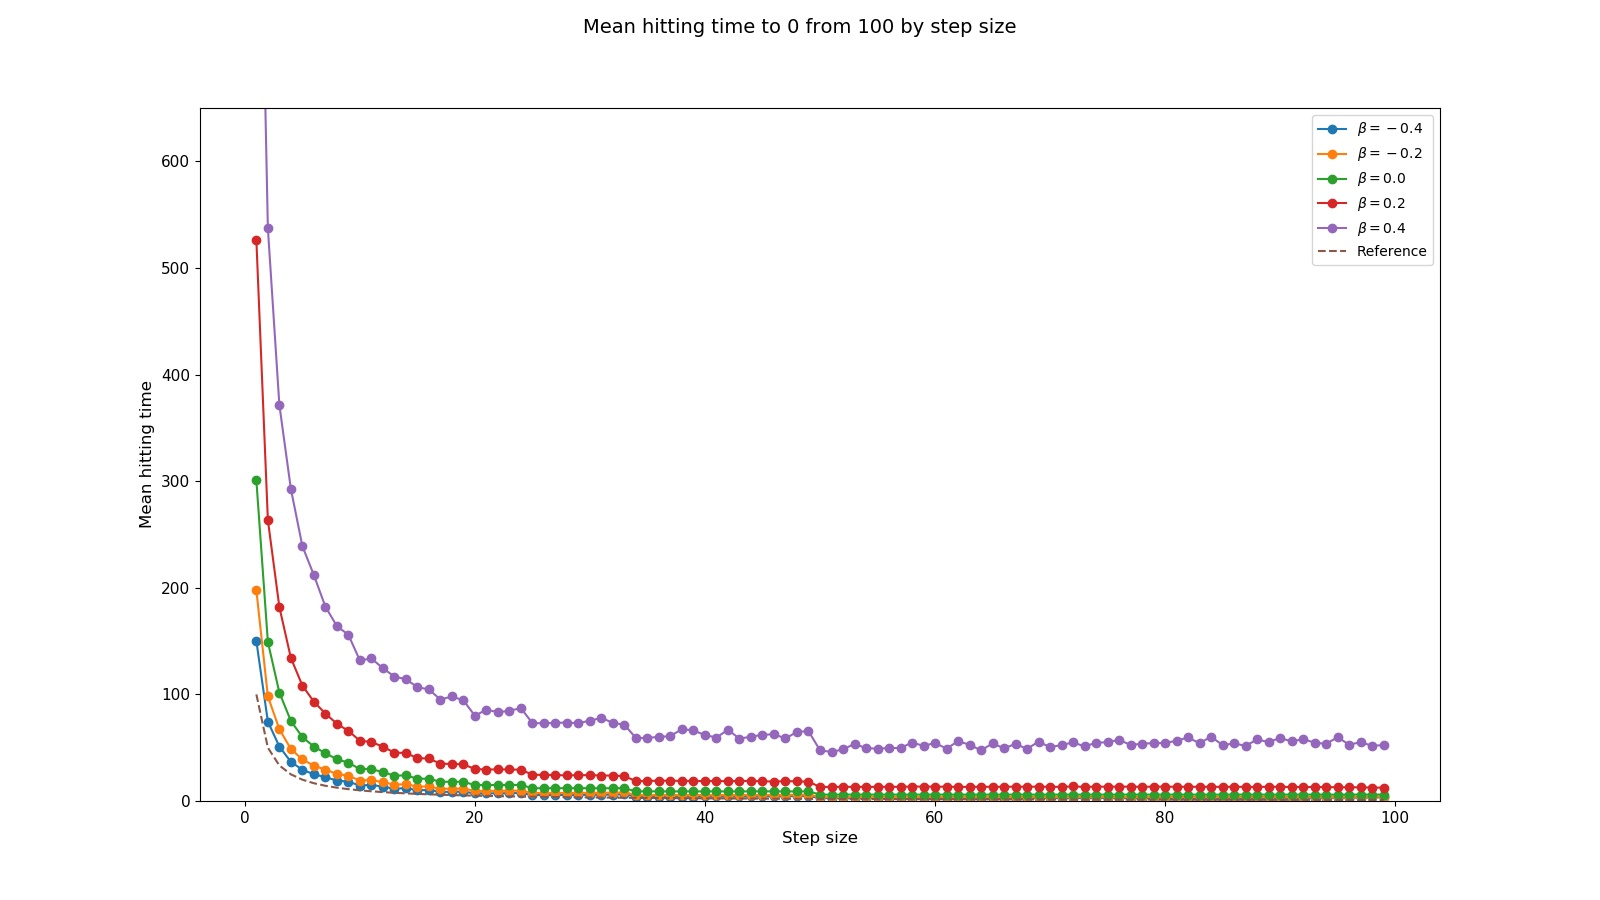
\includegraphics[width=\textwidth]{plots/hittingtimesplot1.jpg}
    \centering
\end{figure}

Further note that a reference data set is also plotted, generated by assuming that $h_s(n) = n/s$, the
``minimal'' scenario. The shape of the resultant plots suggested to me that these hitting time functions
may be scaled versions of the reference scenario, and I set out to further investigate this by
considering the ratio of hitting time functions to the minimal scenario. In other words, I set out to
plot the follwing function:
\[
    \tilde{h}_s(x) = \frac{h_s(x)}{x/s}.  
\]
Doing so in the case of an initial position of $100$ gives the following graph:

\noindent
\begin{figure}[H]
    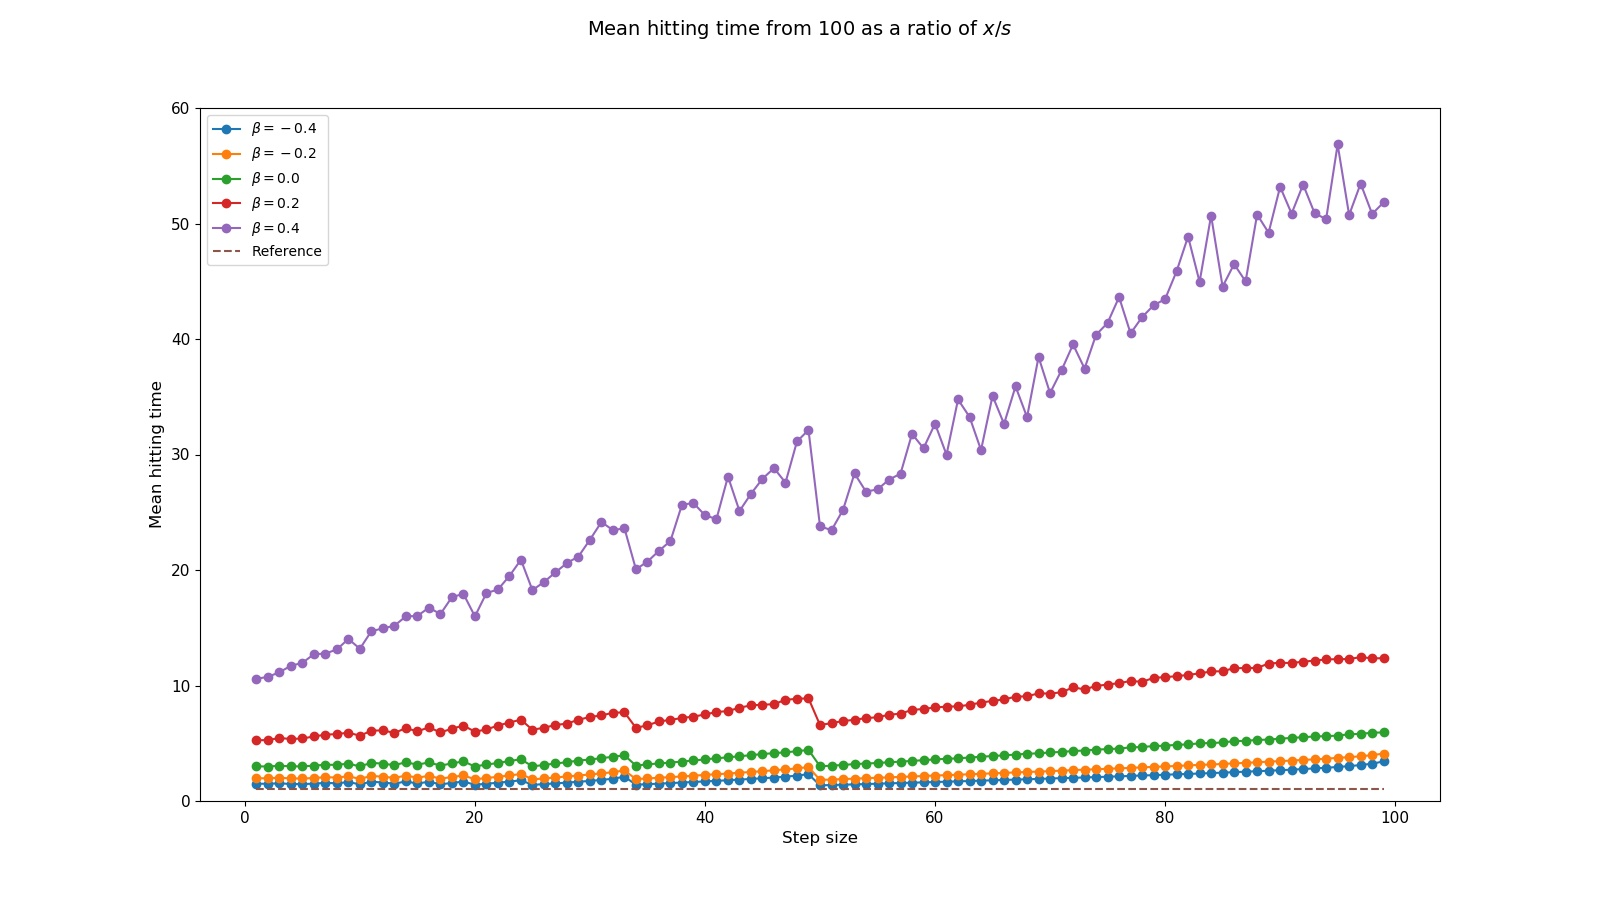
\includegraphics[width=\textwidth]{plots/hittingtimesplot2.jpg}
    \centering
\end{figure}

If the mean hitting time functions were scaled versions of the minimal reference scenario, we would
expect to see lines at constant values (representing the scaling factor). Instead, this plot reveals
that these ratios are generally increasing and so the hitting time functions are not scalings of the
reference scenario. This conclusion is further supported by similar plots generated with an initial
position of $1000$.

However, these plots illuminated an interesting subset of the step sizes where the mean hitting time
seems to instantaneously decrease. I set out to investigate the nature of this sequence, by first
estimating the step-size on the plot. By reading off approximate values, I was able to determine that
this sequence seems to be related to the division algorithm. In particular, we know by the division
algorithm that
\[
    100 = ms + r,
\]
where $s$ represents a step-size, $m$ represents some number of steps, and $r$ represents a remainder
term. Further, the division algorithm guarantees that $r < s$. We hypothesized that if it were also true
that $r < m$, then the corresponding $s$ is a member of this special subset of step-sizes. In the case
of $n=100$, those step-sizes included $50, 33, 25, 20, 16, 14, 12$, and $11$. I then cross-referenced
this sequence with the Online Encyclopedia of Integer Sequences to confirm that this sequence is given
by
\[
    s_{m} = \lf \frac{n}{m} \rf.
\]
However, further pondering led me to believe that this sequence is in fact incorrect. In particular, we
might expect there to be a drop when $s = 34$ instead of when $s = 33$, as it will require at a minimum
$3$ steps to reach $0$ when $s = 34$ as compared to a minimum of $4$ steps when $s = 33$.
Reconsideration of the division algorithm led me to the fact that if the accompanying remainder term is
non-zero, then the walk will have not quite reached the origin in $m$ steps. As a result, the
accompanying step-size is one larger. The sequence when $n=100$ thus instead contains $50, 34, 25, 20,
17, 15, 13$, and $12$. This corresponds to the sequence given by
\[
    s_m = \lc \frac{n}{m} \rc.  
\]

While this sequence of step-sizes was initially of interest due to the instantaneous-behavior, further
investigation led me to deem these sequences unhelpful. It seems that little can be learned about the
behavior of the power-distributed birth and death chain from these sequences.

The investigation of hitting times of the power-distributed chain is also hampered by the fact that when
$\beta > 1$ the mean hitting time may not always be defined. The following plot shows a variety of
different values of $\beta$ (all values less than one are plotted on the left, and all values larger
than one on the right).

\noindent
\begin{figure}[H]
    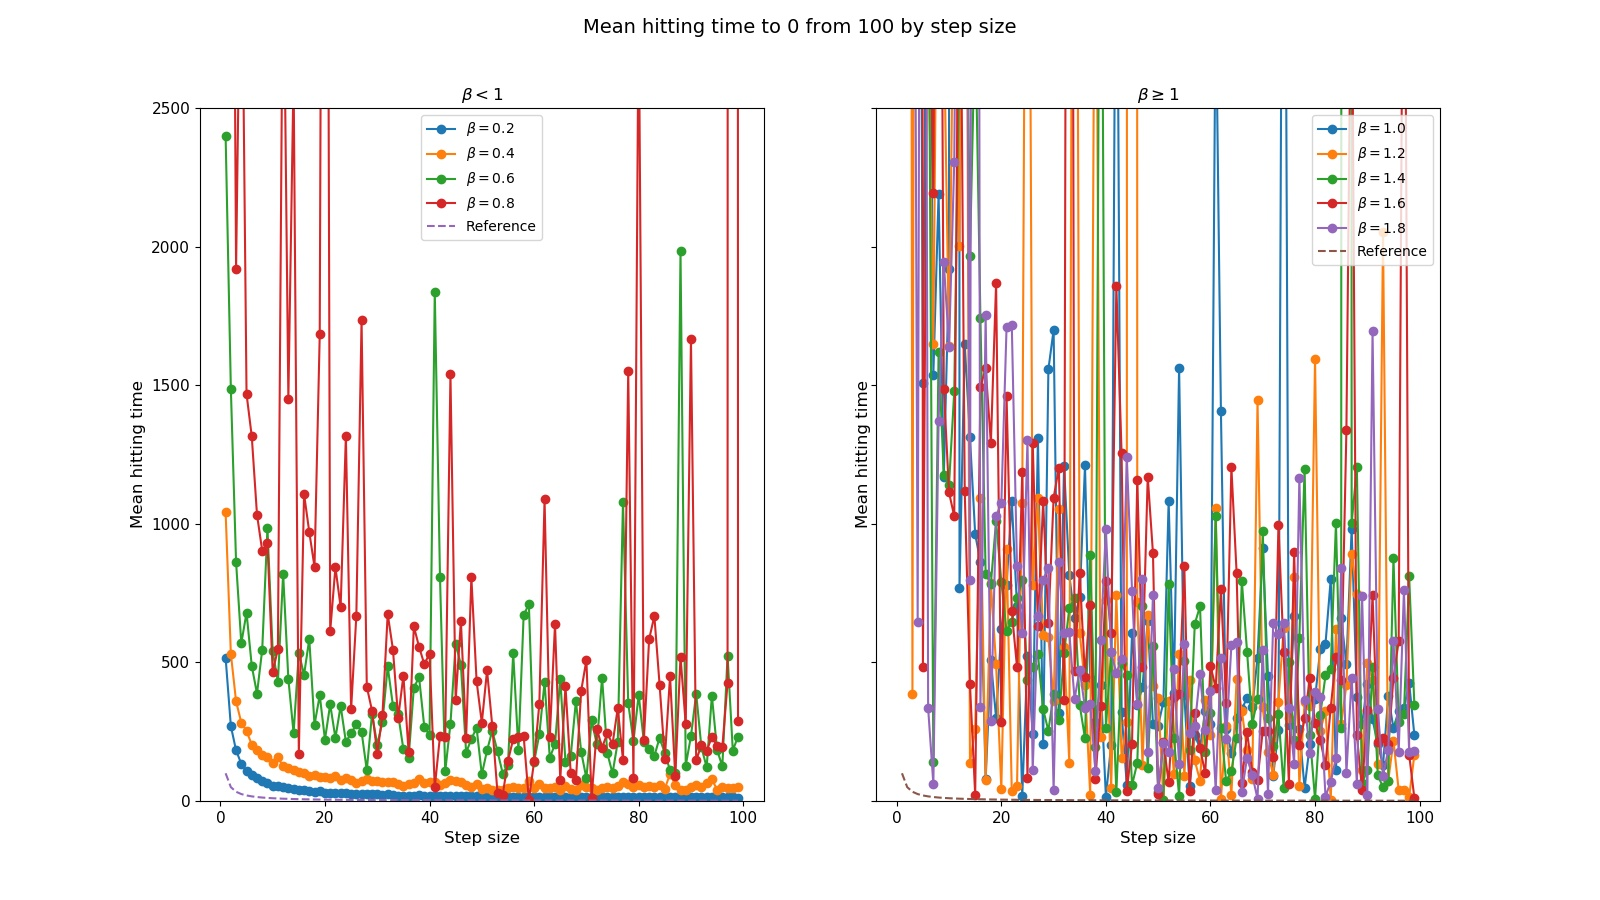
\includegraphics[width=\textwidth]{plots/hittingtimesplot3.jpg}
    \centering
\end{figure}

Notice that on the left, scattering increases greatly as $\beta$ approaches a value of $1$. Further, on
the right, there is scattering for all values of $\beta$ shown. This represents instances where the
simulation diverges away from the origin, not returning with any particular pattern. This is consistent
with the results gathered about return-times of the power-distributed chain when $\beta > 1$.

The results from the simulations on hitting times will next lead me to some analytic investigation of
hitting times. In particular, I would like to begin generalizing some of my results. For example, it may
be true that if the transition probability $p(x)$ monotonically increases to $1/2$ as $x$ approaches
infinity, then the resultant mean hitting time functions $h_s(n)$ behave similarly to the simulated
scenarios.

However, results from the simulations also show that hitting times can only capture so much information
about a given birth and death chain. In the case of the power-distributed chain, mean hitting time
cannot provide useful comparison when $\beta > 1$. As such, further investigation will need to overcome
this obstacle.

\chapter{Further Research}
    As of September 14 and termination of the Northwestern Summer Undergraduate Research Program, I have
completed some investigation into the return times and hitting times from initial position $n$ of the
power-distributed birth and death chain. This leaves open the next steps of this research. A number of
questions remain unanswered. Do monotonically increasing transition probability functions $p(x)$ result
in hitting time functions that resemble those generated by the power-distributed chain? How do we
compare chains in which the mean hitting time is not defined (in other words, how do we compare chains
that seem to ``get lost'')?

Perhaps the most important next step of research will involve generalizing some of the results gathered
here. The power-distributed chain is but one chain out of an infinite number of possibilities, and
finding the best way to compare arbitrary chains is critical to developing a complete theory of
mathematical fragility. It may make the most sense to investigate the probability that a birth and death
chain with initial position $n$ and step size $s$ will reach the origin, as this quantity should be
defined for all chains. This will allow comparison of chains where the mean hitting time diverges, like
in the case of the power-distributed chain when $\beta$ is larger than $1$.

To this end, continuing to update simulations to test new parameters and transition probabilities will
help guide intuitions. However, the desire to move into cases of more generality will need more analytic
methods. Hopefully I can continue to develop my investigation into more complex forms of analysis,
perhaps making heavy use of sequences and limiting behavior. While the work presented here is just the
beginning of development of mathematical fragility, I hope to broaden my investigation to generate more
interesting results. Further, I hope that this project will be able to follow my mathematical education.
As I continue to learn techniques from various different fields, I would like to apply these to this
project.


\end{document}
